\documentclass{article}

\PassOptionsToPackage{numbers, compress}{natbib}

\usepackage[final]{neurips_2024}

\usepackage[utf8]{inputenc}
\usepackage[T1]{fontenc}
\usepackage{hyperref}
\usepackage{url}
\usepackage{booktabs}
\usepackage{amsfonts}
\usepackage{nicefrac}
\usepackage{microtype}
\usepackage{xcolor}
\usepackage{graphicx}
\usepackage{float}
\usepackage{subfig}
\usepackage{amsmath}
\usepackage{amssymb}
\usepackage{cleveref}

\title{Revisiting Uniform Information Density: A Public Replication and Extension Study}

\author{%
  Zitong Luo \\
  Center for Data Science\\
  New York University\\
  \texttt{zl5847@nyu.edu} \\
  \And
  Qianqian Zhao \\
  Center for Data Science\\
  New York University\\
  \texttt{qz2671@nyu.edu} \\
}

\begin{document}

\maketitle

\begin{abstract}
The uniform information density (UID) hypothesis proposes that speakers tend to distribute information so that surprisal remains approximately even across an utterance. Here we replicate Meister et al.'s study of the UID hypothesis on a public data subset and add three extensions: OneStop (ordinary eye-tracking), MegaAcceptability (clause-embedding judgments), and EMTeC (eye movements on LLM-generated text). The public replication is consistent with the original qualitative contrast: acceptability judgments show clearer benefits from non-linear surprisal predictors than reading-time data. Scoring every extension with GPT-2, BERT, and a WikiText-103 5-gram model sharpens this contrast but also exposes model dependence: MegaAcceptability gives the clearest acceptability-side generalization, EMTeC gives a small reading-time signal, and OneStop remains weak at the paragraph level.
\end{abstract}

\section{Introduction}

Information theory gives a compact way to connect linguistic prediction with human processing. The surprisal of a word $u_n$ is $s(u_n)=-\log p(u_n \mid u_{<n})$, so lower-probability words carry more information \cite{shannon1948,hale2001,levy2008}. Prior literature work shows that contextual surprisal predicts processing difficulty is approximately linear \cite{smithLevy2013,goodkind2018}. UID posits a related but stronger efficiency claim: speakers avoid sharp peaks and troughs in information density \cite{levyJaeger2007}. Our goal is to test whether this efficiency claim extends beyond production to comprehension and acceptability judgments.

Meister et al. \cite{meister2021} made this issue testable by comparing a family of sentence-level predictors:
\begin{equation}
  C_k(u)=\sum_{n=1}^{N} s(u_n)^k .
  \label{eq:power}
\end{equation}
When $k=1$, this reduces to summed surprisal, matching the standard additive surprisal account. When $k>1$, high-surprisal words receive disproportionate weight; for fixed total information and length, such a cost is minimized by more uniform information allocation. Meister et al. report that reading-time data are broadly consistent with previous linear surprisal results, but also compatible with weak super-linearity, whereas acceptability judgments more clearly favor $k>1$ and other global UID operationalizations.

Our project asks whether this prior result is reproducible and whether its boundary conditions are theoretically meaningful. Our replication focus on public data subset: CoLA \cite{warstadt2019} and BNC acceptability judgments \cite{lau2017}, Natural Stories self-paced reading \cite{futrell2018}, Provo eye movements \cite{luke2018}, GPT-2 \cite{radford2019}, BERT \cite{devlin2019}, and a WikiText-103/KenLM 5-gram model \cite{merity2017,heafield2011}. We then ask whether the same UID logic transfers to ordinary reading, structured acceptability, and reading of LLM-generated text using OneStop \cite{berzak2025}, MegaAcceptability \cite{whiteRawlins2020}, and EMTeC \cite{bolliger2025}.

\section{Methods}

\textbf{Replication scope.} We adapted the original public repository released by Meister et al. \cite{meister2021}. The public workflow reproduces the analyses that can be rerun without restricted access: CoLA, BNC, Natural Stories, Provo, UCL auxiliary data, and WikiText-103. Brown is unavailable because the original Google Drive archive currently fails; Dundee requires separate access; GECO is optional and not part of the public rerun; and TransfoXL was skipped because its upstream Hugging Face path is deprecated in our environment.

\textbf{Predictors and models.} For each sentence, we computed token-level or word-level surprisal estimates and aggregated them with \cref{eq:power} over a grid of $k \in \{0.25,0.5,\ldots,2.75\}$. GPT-2 supplies autoregressive neural surprisals, BERT supplies pseudo-surprisals, and KenLM supplies a 5-gram baseline trained on WikiText-103. For reading-time datasets, the dependent variable is sentence-level reading time aggregated over words; for acceptability datasets, the dependent variable is the sentence acceptability label or score.

\textbf{Evaluation and extension design.} Each UID predictor is added to a baseline regression and evaluated by held-out $\Delta$LogLik; positive values mean higher held-out likelihood. The extensions keep the same power sweep and scoring families as the main replication: GPT-2, BERT, and KenLM. Controls are adapted to each corpus: OneStop uses paragraph length and word frequency; MegaAcceptability uses length, verb identity, and syntactic frame; EMTeC uses grouped folds by generated-text condition and controls for length, lexical frequency, subject, generator model, decoding strategy, and task. Because the extension runner was AI-assisted, we verified its UID feature math and CV recovery on simulated data before applying it to real corpora.

\section{Results}

\begin{figure}[t]
  \centering
  \subfloat[Power sweep.]{
    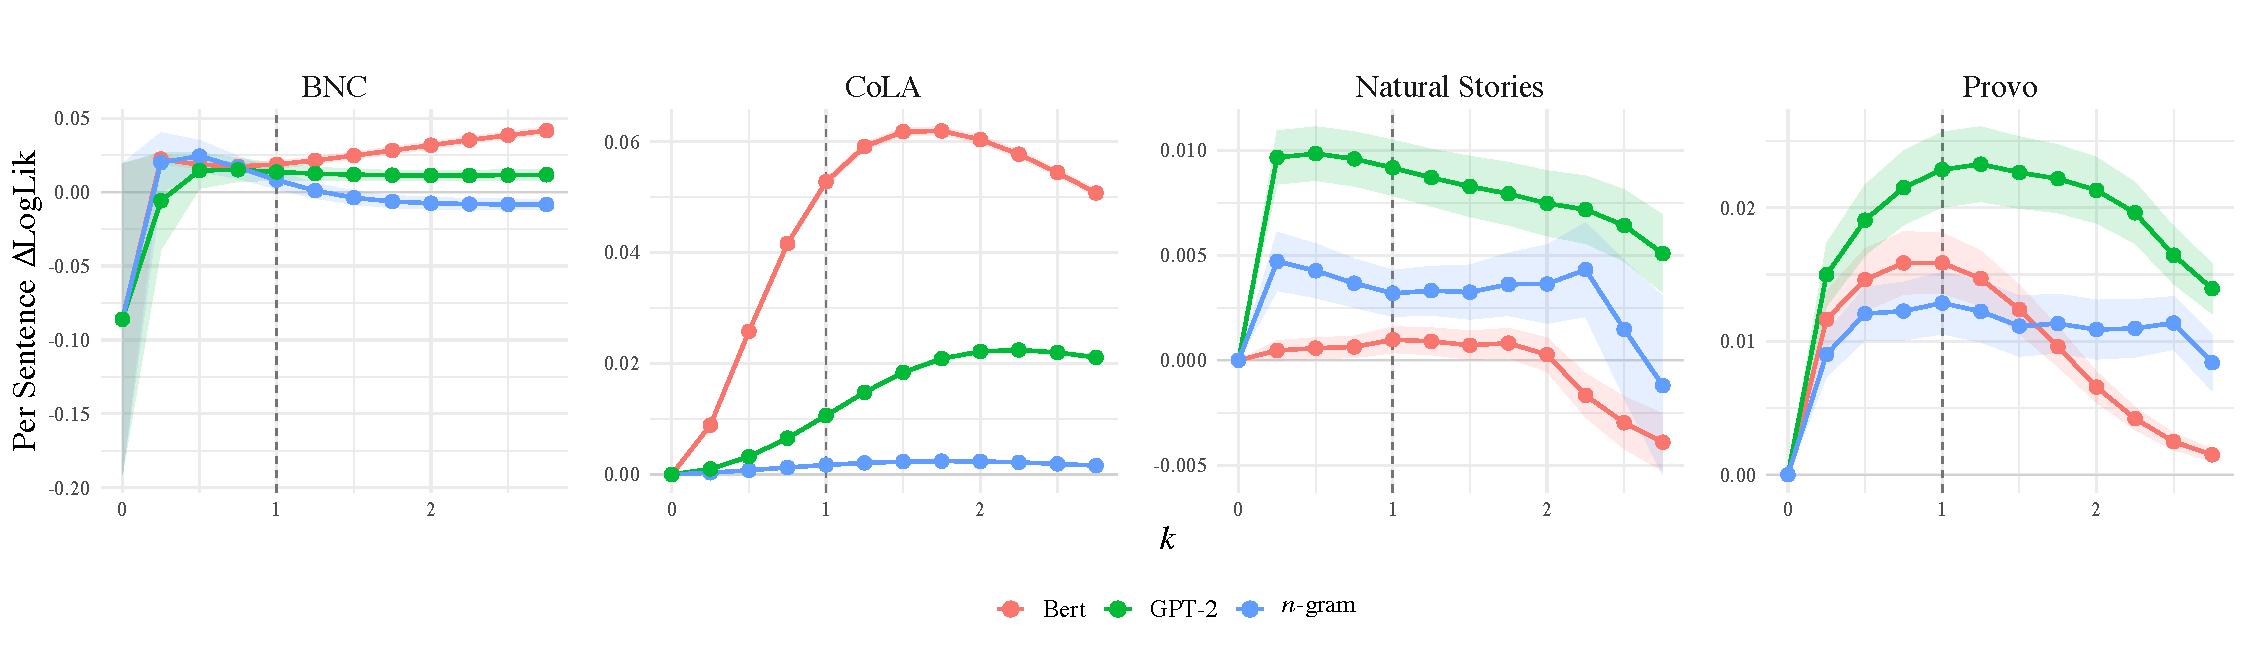
\includegraphics[width=0.96\linewidth]{graph/figure_reading_acceptability_delta_loglik.pdf}
  }\\[-0.25em]
  \subfloat[Acceptability correlation.]{
    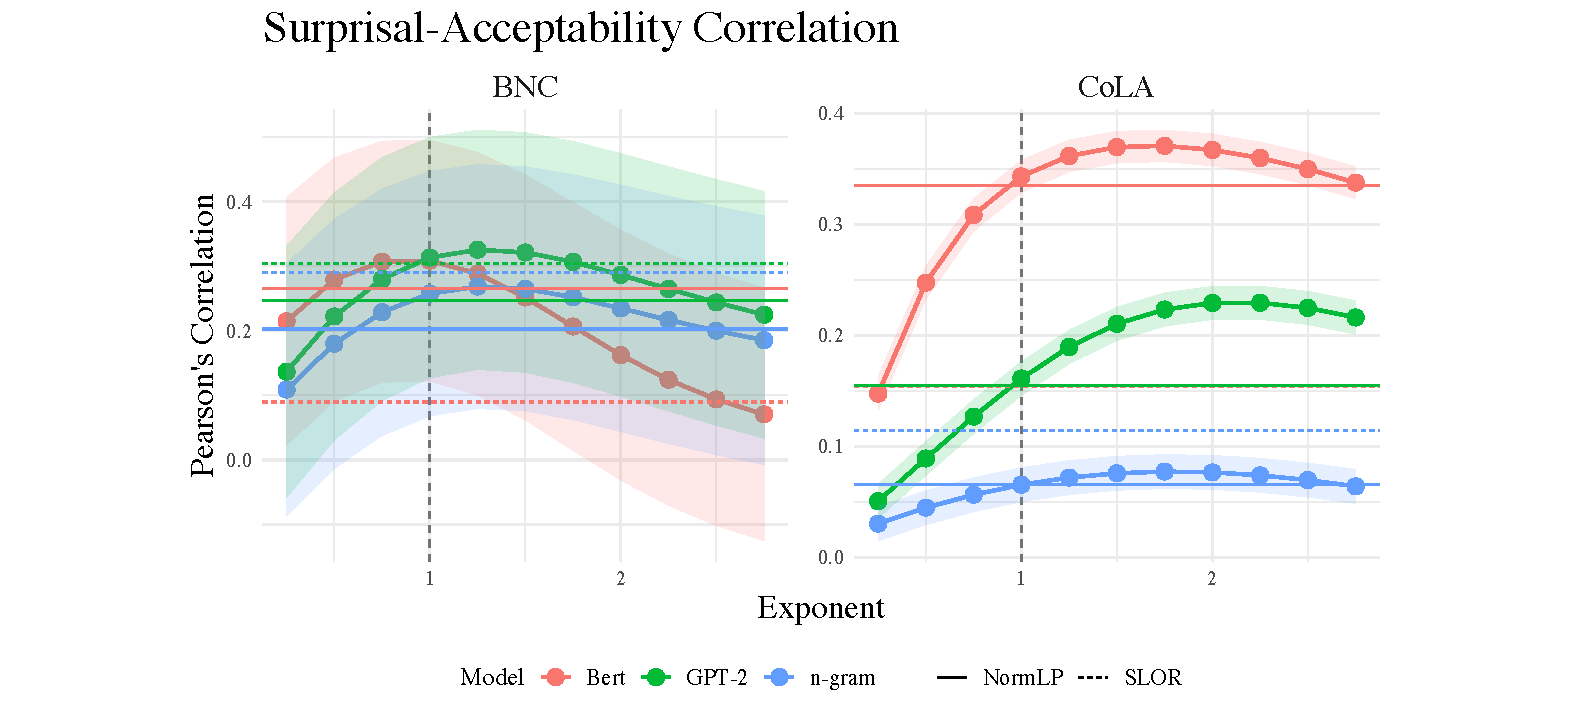
\includegraphics[width=0.58\linewidth]{graph/figure_surprisal_acceptability_correlation.pdf}
  }
  \caption{Public replication diagnostics. The main power sweep compares reading-time and acceptability datasets, while the correlation panel checks whether transformed surprisal is directly associated with graded acceptability.}
  \label{fig:main}
\end{figure}

\textbf{Main replication.} \Cref{fig:main} recovers the main qualitative asymmetry in Meister et al. \cite{meister2021}. Public reading-time results do not strongly reject the linear $k=1$ account: Provo peaks at $k=1$ for BERT and the 5-gram model, and only $k=1.25$ for GPT-2, with a very small gain over $k=1$ ($0.0004$ held-out log-likelihood per observation). Natural Stories is similarly weak. Acceptability is more sensitive to non-linear information-density costs: in CoLA, all three model families peak above $1$, and in BNC, BERT peaks at $k=2.75$. The correlation panel gives the same message without a regression baseline. Thus, the replicated contrast is that acceptability judgments are more sensitive than reading times to the shape of the surprisal distribution.

\begin{figure}[t]
  \centering
  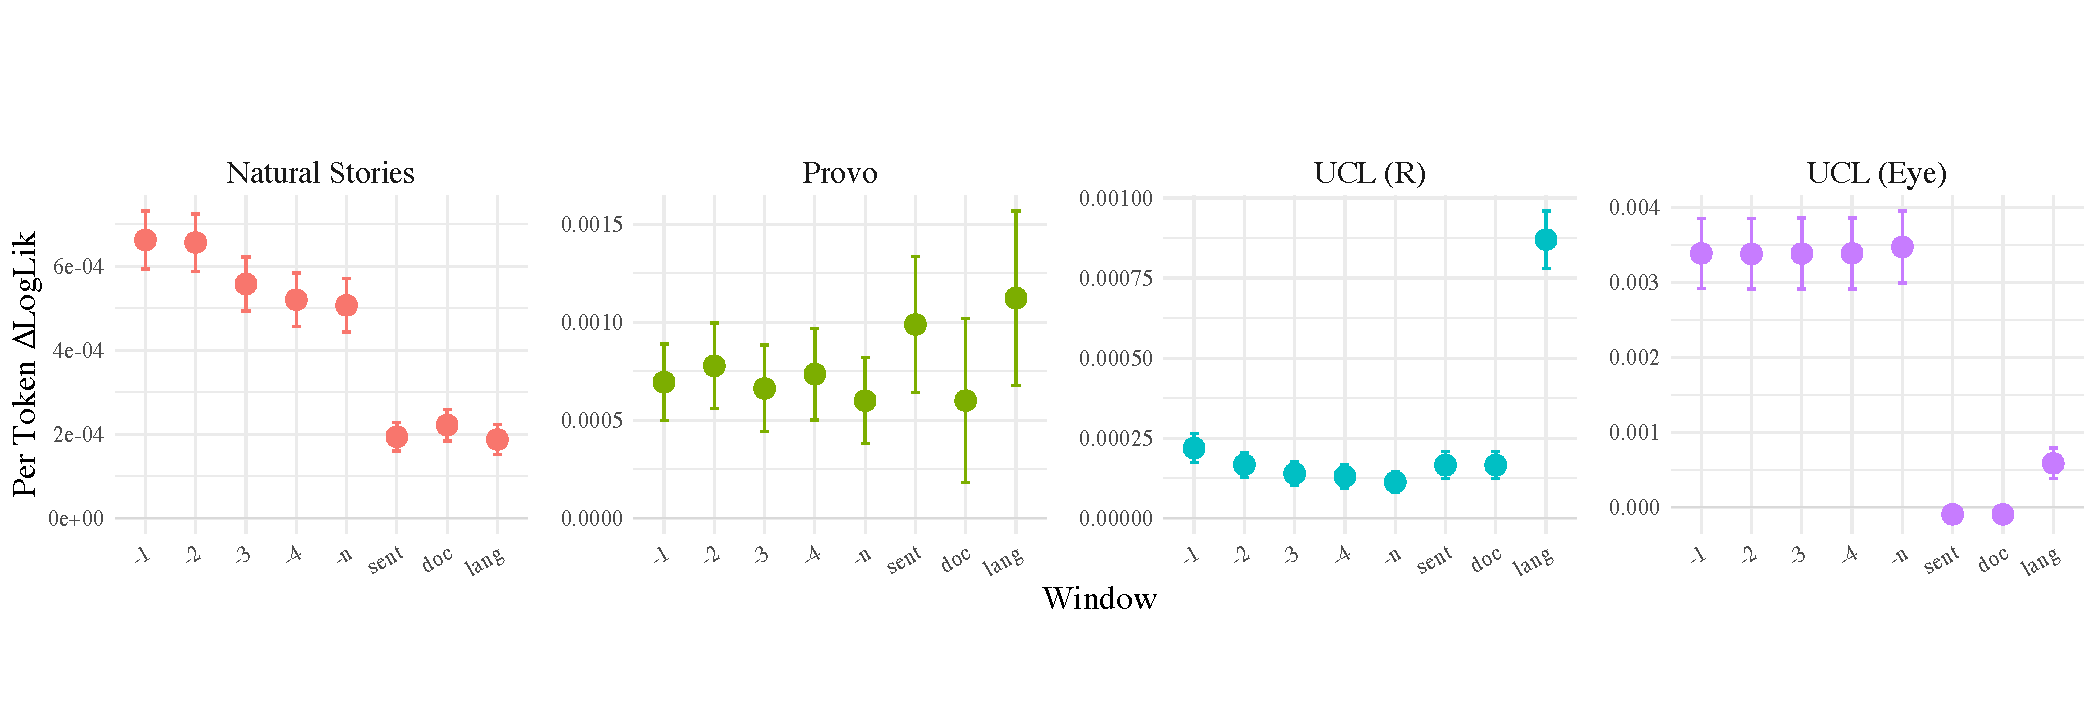
\includegraphics[width=0.95\linewidth]{graph/figure_case_study3_windows.pdf}
  \caption{Replication of the windowed UID analysis. The public data show small differences across local and broader context windows, supporting a cautious interpretation of scope effects in the public subset.}
  \label{fig:windows}
\end{figure}

\textbf{Scope of UID pressure.} \Cref{fig:windows} checks whether UID should be operationalized locally, over adjacent words, or over broader contexts. The public version is less decisive than the original because several reading corpora are unavailable, but the small window differences reinforce the main message: acceptability-side non-linearity is more robust than fine-grained claims about the exact context window.

\begin{figure}[t]
  \centering
  \subfloat[Extension 1: OneStop.]{
    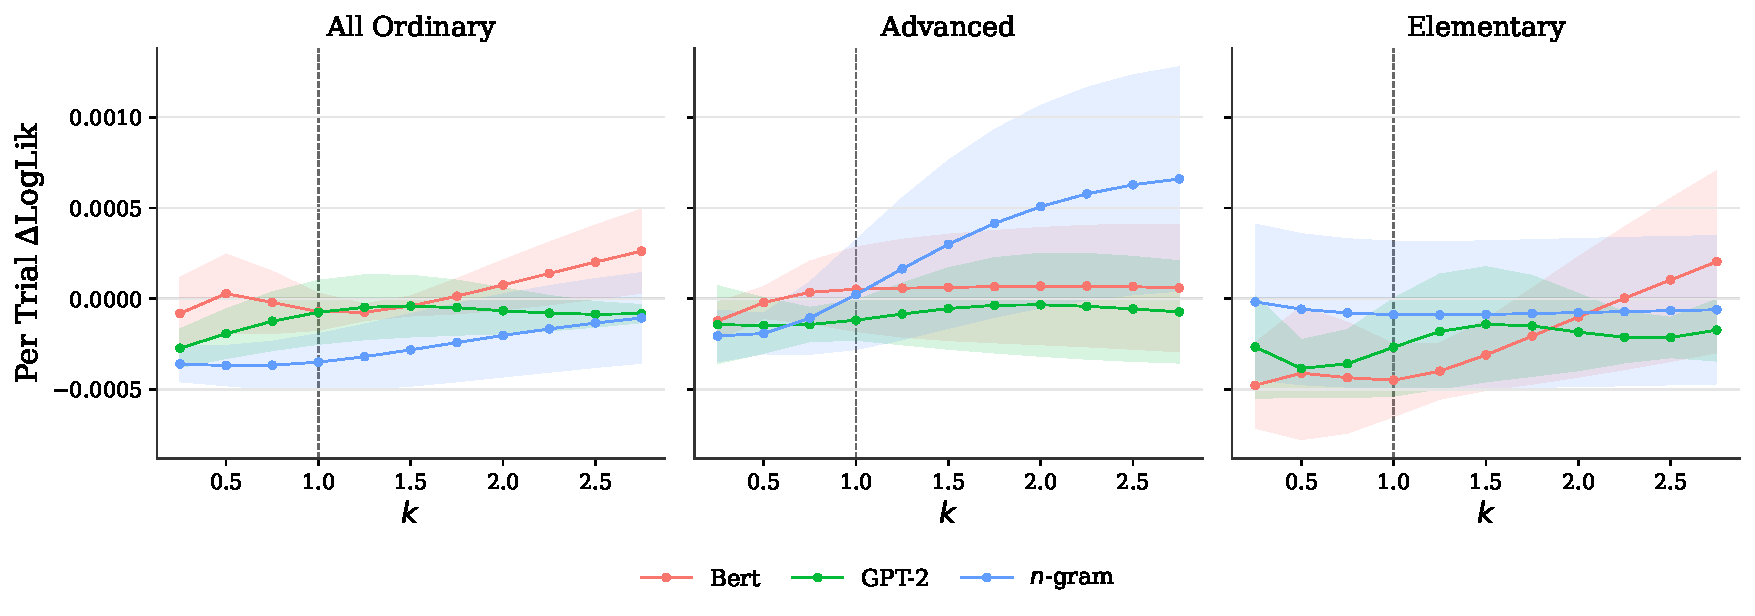
\includegraphics[width=0.47\linewidth]{graph/figure_onestop_ordinary_uid_by_difficulty.pdf}
  }
  \hfill
  \subfloat[Extension 2: MegaAcceptability.]{
    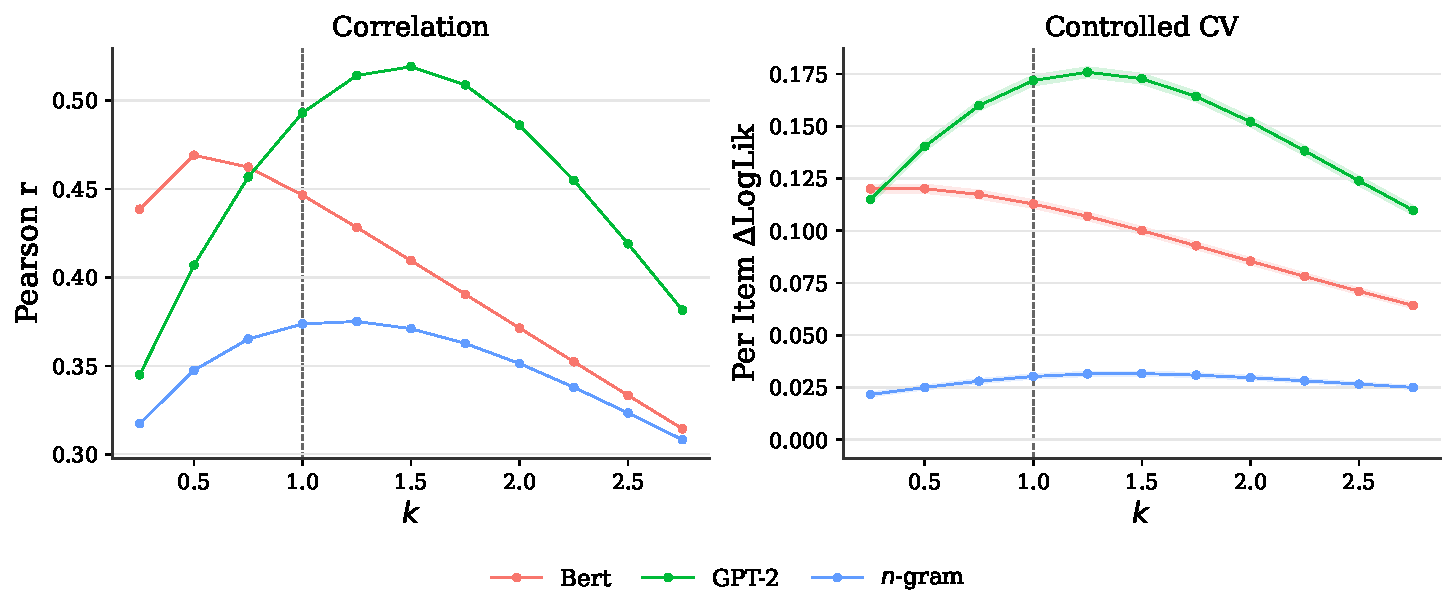
\includegraphics[width=0.47\linewidth]{graph/figure_mega_acceptability_uid_power_sweep.pdf}
  }\\[-0.25em]
  \subfloat[Extension 3: EMTeC.]{
    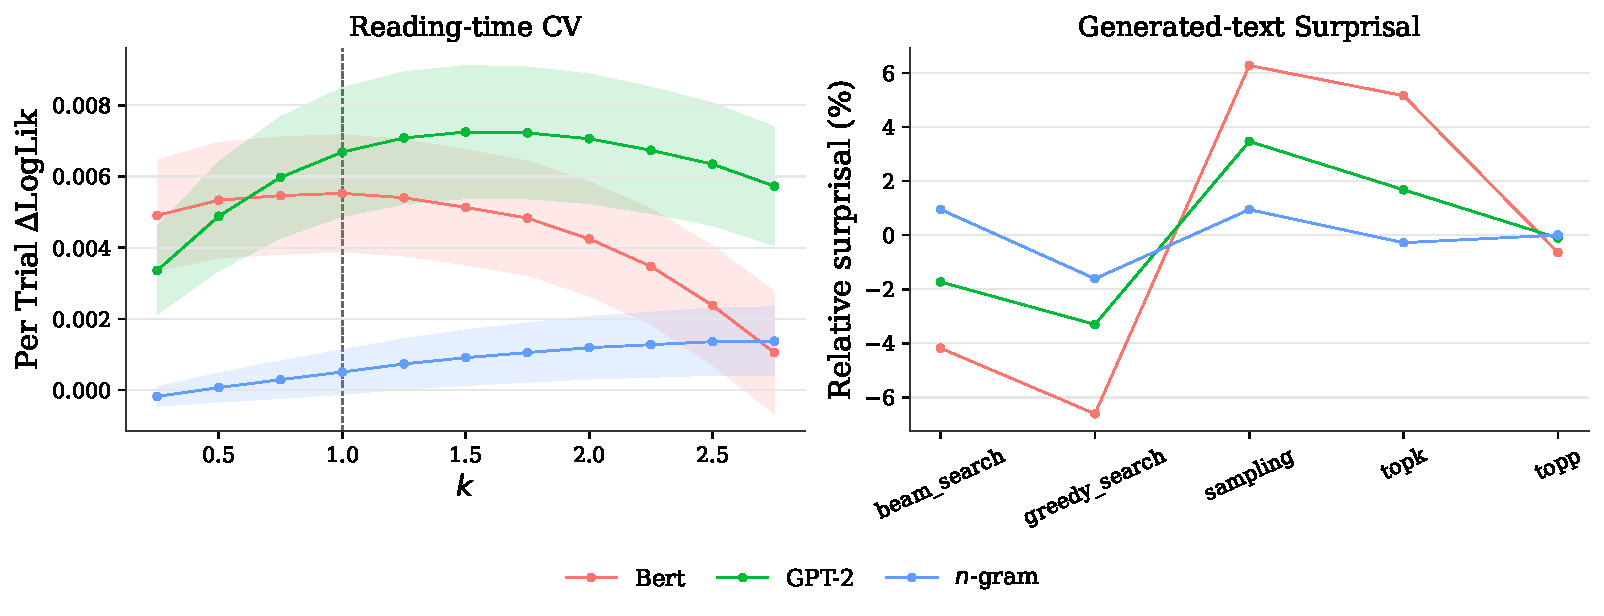
\includegraphics[width=0.74\linewidth]{graph/figure_emtec_uid_generated_text.pdf}
  }
  \caption{Extension analyses. Each extension is scored with GPT-2, BERT, and a WikiText-103 5-gram model. OneStop tests ordinary paragraph eye-tracking, MegaAcceptability tests clause-embedding acceptability, and EMTeC tests eye movements over LLM-generated text.}
  \label{fig:extensions}
\end{figure}

\textbf{Extensions.} \Cref{fig:extensions} asks whether UID effects are broad or dataset-specific across ordinary reading, acceptability, and generated text.

\textbf{Extension 1: OneStop.} OneStop is a reading-time/eye-tracking dataset like the original paper's reading-time corpora, but it uses ordinary reading passages and includes text difficulty levels. Its objective is to test whether UID effects generalize to a new eye-tracking corpus and vary across difficulty. The result is cautious. All Ordinary peaks at $k=2.75$ for BERT ($\Delta$LogLik $=0.00026$), $k=1.5$ for GPT-2 ($-0.00004$), and $k=2.75$ for the 5-gram model ($-0.00011$). Advanced texts show a small positive 5-gram peak at $k=2.75$ ($0.00066$), but signs and magnitudes vary across models and subsets. The paragraph-level OneStop extension therefore does not provide a robust ordinary-reading generalization of the acceptability-side UID pattern.

\textbf{Extension 2: MegaAcceptability.} MegaAcceptability is an acceptability judgment dataset like CoLA/BNC, but it provides finer normalized ratings for clause-embedding verbs across syntactic frames. Its objective is to test whether the acceptability-side UID effect generalizes beyond broad or binary judgments to syntactic/semantic acceptability. This remains the strongest extension result, but the three-model rerun makes the claim more precise. GPT-2 peaks above linearity in both diagnostics: $k=1.25$ in controlled CV ($\Delta$LogLik $=0.1759$) and $k=1.5$ in correlation ($r=0.519$). The 5-gram model also peaks above linearity: $k=1.5$ in CV ($0.0316$) and $k=1.25$ in correlation ($r=0.375$). BERT is strongly predictive but peaks at $k=0.5$ in both diagnostics ($\Delta$LogLik $=0.1201$, $r=0.469$). Thus, MegaAcceptability supports an acceptability-side surprisal effect beyond lexical and frame controls, while the preferred exponent is model-dependent rather than uniformly super-linear.

\textbf{Extension 3: EMTeC.} EMTeC is also a reading-time/eye-tracking dataset, but it uses LLM-generated texts produced by different models and decoding strategies. Its objective is to test whether UID effects generalize to human reading of generated text and whether decoding strategies produce different UID profiles. The reading-time gain is small and model-dependent: GPT-2 peaks at $k=1.5$ ($\Delta$LogLik $=0.00725$ versus $0.00669$ at $k=1$), BERT peaks at the linear $k=1$ setting ($0.00553$), and the 5-gram model peaks at $k=2.75$ but with a smaller effect ($0.00138$). The normalized decoding-strategy panel compares each scoring model against its own mean; sampling and top-$k$ are relatively high-surprisal, while greedy search is relatively low-surprisal, especially under BERT and GPT-2. Generation strategy therefore changes the information-density profile readers encounter, even though the reading-time evidence remains modest.

\section{Discussion}

Our project has two main goals: first, to replicate Meister et al.'s study of the UID hypothesis; second, to add three extensions that test the generalizability of UID to new tasks and text types. It is interesting to see a consistent pattern across our results: acceptability always shows stronger UID effects than reading time. This replicates the original paper's main contrast. But we also see that effect strength varies by task and text type. MegaAcceptability strengthens the acceptability-side conclusion, OneStop remains near zero at the paragraph level, and EMTeC shows only small reading-time gains.

Our approach matters because it tests the boundaries of UID beyond the original datasets. By applying the same three model families to every extension, we can compare results across tasks and corpora directly. This lets us see where UID generalizes (MegaAcceptability), where it weakens (OneStop), and where it gives mixed signals (EMTeC). The significance is to understand it as a context-dependent principle.

For future exploration, we can test more languages and spoken language data. Current work covers only English and Dutch, and only written text. We can also apply word-level mixed-effects models. These models allow us to control for two sources of noise: subject variability (some people read faster than others) and word variability (short words require less time to process than longer ones). By predicting reading time for each word, we could better detect whether surprisal spikes at specific words drive the UID effect.

\clearpage

\section*{Data and code availability statement}

This replication is based on the public code release for Meister et al. \cite{meister2021}: \url{https://github.com/rycolab/revisiting-uid}. Our course repository contains the reproducible public-data workflow, scripts, notebooks, compact checkpoint CSVs, and figures: \url{https://github.com/luozt20/Revisiting-the-Uniform-Information-Density-Hypothesis-A-Replication-Study}. The main public replication notebook is \texttt{src/revisiting-uid-public.ipynb}; the three extension analyses are run by \texttt{src/extension\_three\_model\_analysis.py}; and simulated-data checks for AI-assisted analysis code are run by \texttt{src/verify\_ai\_assisted\_analysis.py}. GPT-2 and BERT scores were computed through Hugging Face Transformers \cite{wolf2020}. Figures used in this report were generated by repository code, not by AI image/table generation, and copied from \texttt{src/figures/} into \texttt{Project Report LaTeX/graph/}. Dataset sources and licenses are those of the cited dataset creators.

\section*{Author contribution statement}

Qianqian Zhao led data preparation and the experiment pipeline: dataset organization, preprocessing, tokenization, language-model setup, public workflow scripts, and reproducibility checks. Zitong Luo led analysis and visualization: surprisal extraction, UID metric computation, statistical comparisons, figure generation, and interpretation of results. Both authors contributed to literature review, report writing, proofreading, and final check.

\section*{AI usage statement}

The authors used ChatGPT/Codex as a supportive assistant for codebase inspection, README/report organization, proofreading, LaTeX compilation debugging, plotting-code cleanup, and boilerplate/scaffolding for the public workflow and three-model extension runner. AI tools were not used to generate experimental stimuli, fabricate data, invent results, draft substantive report text, or create final figures directly; all report figures were generated by repository code from cited datasets and checkpoint CSVs. The authors checked factual claims against repository outputs and cited sources, read and tested the AI-assisted code, and ran the simulated-data verification script \texttt{src/verify\_ai\_assisted\_analysis.py}. The authors remain responsible for the final code, citations, and scientific claims.

\section*{Acknowledgments}

We thank the course instructor Noga Zaslavsky and teaching assistant Moufan Li for guidance and Meister et al. for releasing the original UID analysis code. We especially thank our professor for feedback after our presentation; in response, we revised the extension analyses so that each extension uses the same GPT-2, BERT, and WikiText-103 5-gram scoring families used in the main replication, which made the extension results more complete and easier to compare. We also acknowledge the creators of the public datasets and tools cited in this report.

\bibliographystyle{unsrtnat}
\bibliography{refs}

\end{document}
